\Chapter{Tervezés}
Ebben a fejezetben a web alkalmazás kinézetéről és adatmoteljéről lesz szó.

Terveséhez az Uizard\cite{uizard} nevű oldalt használtam.

\Section{A feladatom}

A feladatom egy olyan webalkalmazás fejlesztése, amely alkalmas más oldalak autó hirdetéseinek aggregálására és az autók böngészésére. Alkalmazás funkciói:

\begin{itemize}
\item Regisztráció, a felhasználó végzi el felhasználónév és jelszó pár megadásával.
\item Felhasználó jogosultságának mosósítása:
	\begin{itemize}
	\item Admin: mindenhez hozzá fér, ő frissíti az elérhető autókat, felhasználók jogosultságát változtatja, és törölheti a felhasználót.
	\item User: a hirdetése és a statisztika megtekintésére jogosult.
	\end{itemize}
\item Hirdetések megtekintése, ahol az oldalon megtalálható autókat tudjuk megtekinteni.
\end{itemize}

\Section{Kinézet és felépítés}

A kinézet minél felhasználó barátiabb lesz, hogy felhasználók minél könnyebben tudják majd használni az alkalmazást

\subsection{Regisztráció és bejelentkezés}

Ha már van fiókunk az oldalhoz, akkor a felhasználónév és a jelszó megadása után be is tudunk jelentkezni az oldalra

\newpage

\begin{figure}[h]
\centering
\fbox{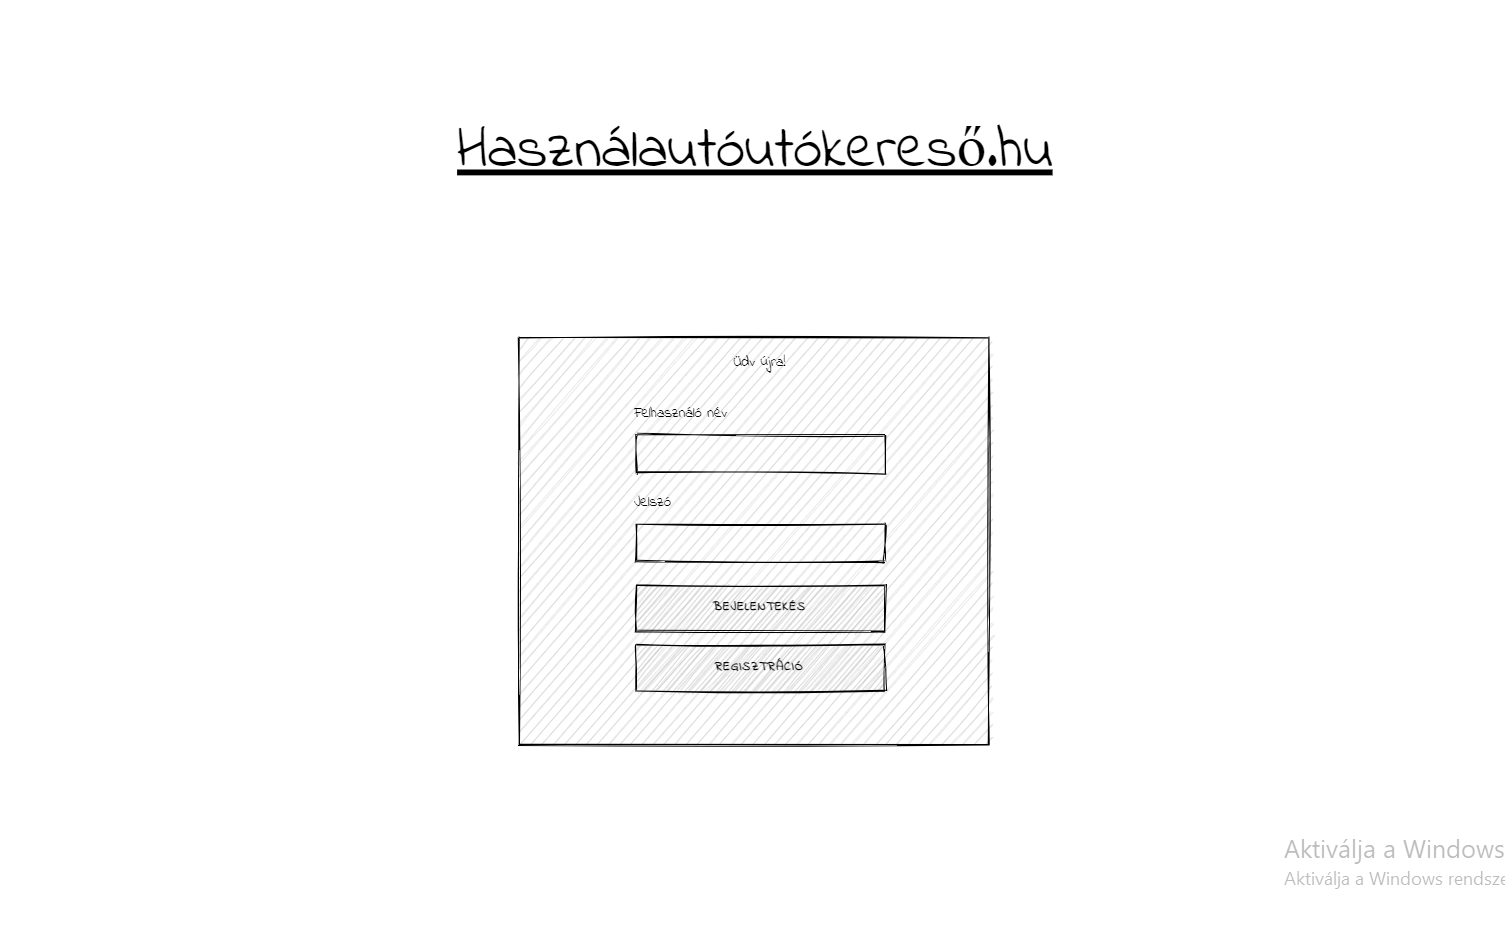
\includegraphics[scale=0.4]{images/login.png}}
\caption{Bejelentkezés}
\label{fig:Bejelentkezés}
\end{figure}

Regisztrációs felületen a felhasználónév és jelszó megadása után be tudunk regisztrálni és máris tudjuk használni a weboldalt

\begin{figure}[h]
\centering
\fbox{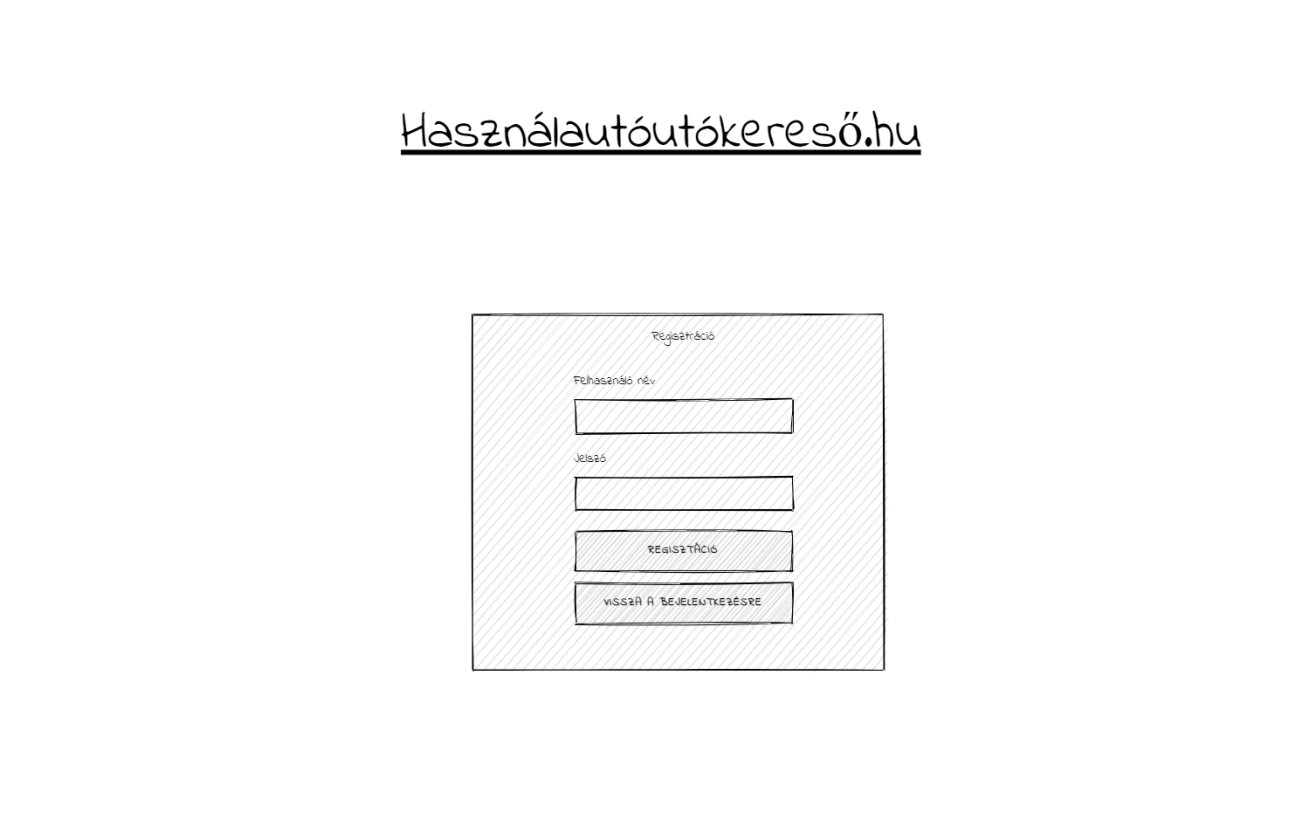
\includegraphics[scale=0.8]{images/register.png}}
\caption{Regisztráció}
\label{fig:Regisztráció}
\end{figure}

\newpage
\subsection{Főoldal}

A főoldalon látunk egy szűrő felületet, ahol ki lehet választani, hogy milyen márkájú és modellű autót milyen üzemanyag használattal, milyen évjárat és hengerűrtartalom között szeretnénk keresni, van lehetőség az ár sáv megadására is.

Látunk, egy diagramot ahol statisztikát tudunk megtekinteni az autókra keresések számáról.

\begin{figure}[h]
\centering
\fbox{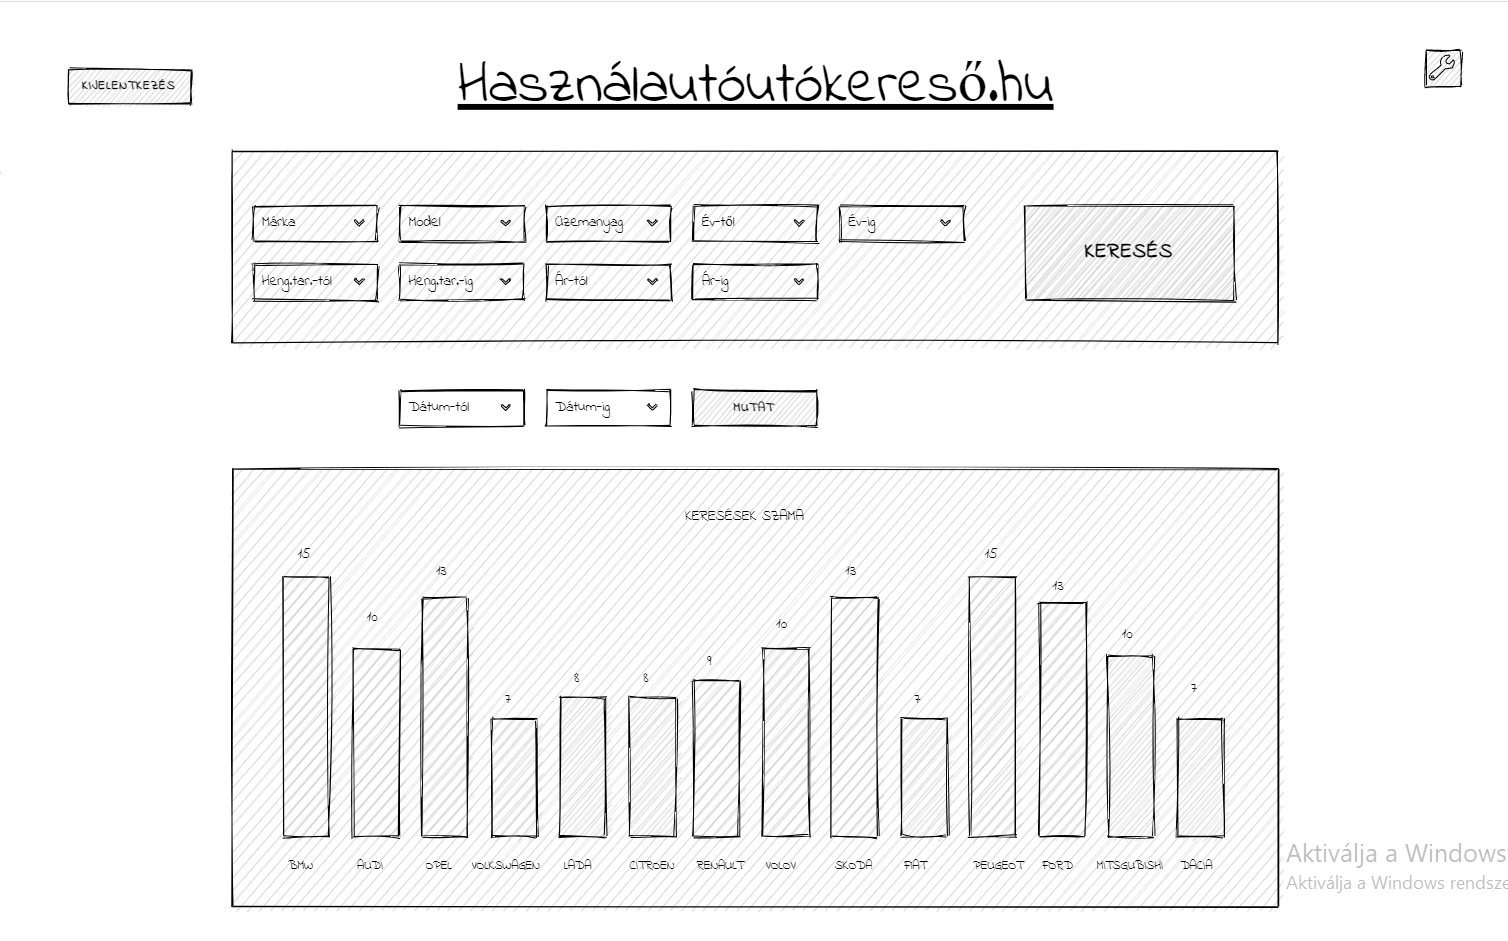
\includegraphics[scale=0.4]{images/Fooldal.png}}
\caption{Főoldal}
\label{fig:Fooldal}
\end{figure}

Van egy csavarkulcs is, amit csak ADMIN felhasználó lát.

\subsection{Találatok megtekintése}

A találati oldalon láthatjuk az autókat, egy képet az autóról, az alap információkat, mint évjárat, ló erő, vagy a köbcenti.

Ha megtaláljuk a megfelelő autót, akkor a megnézem, gombra kattintva meg is tudjuk tekinteni az autót.
\newpage

\begin{figure}[h]
\centering
\fbox{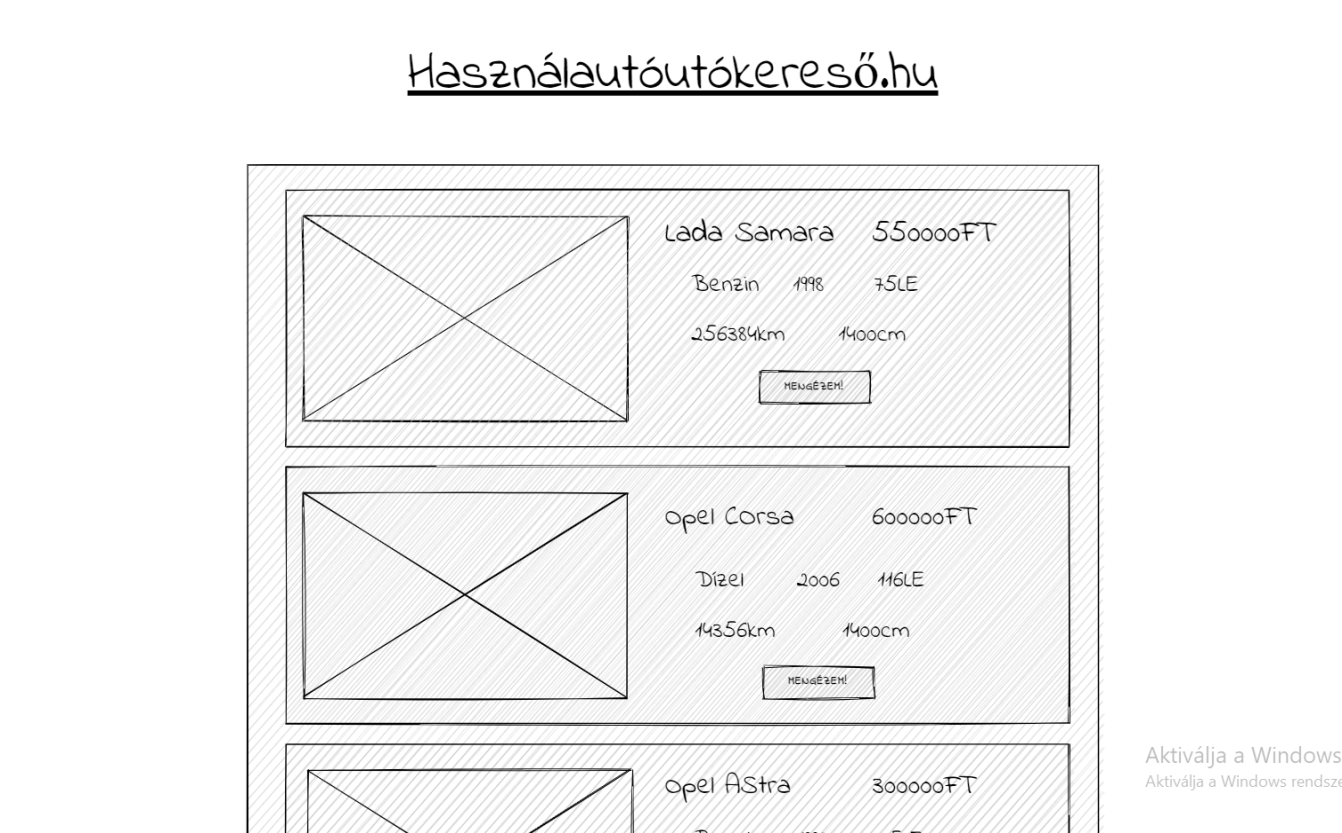
\includegraphics[scale=0.8]{images/Talalatok.png}}
\caption{Találati oldal}
\label{fig:Talalatok}
\end{figure}

\subsection{Admin oldal}

Az Admin oldalon találunk egy táblázatot a felhasználókról, ami tartalmazza a felhasz-
náló nevet és a jogosultságot. Jogosultságot itt tudjuk módosítani Admin is User között.

Itt van lehetőség törölni a felhasználókat vagy az autók lekérdezésére a többi webol-
dalról.

\begin{figure}[h]
\centering
\fbox{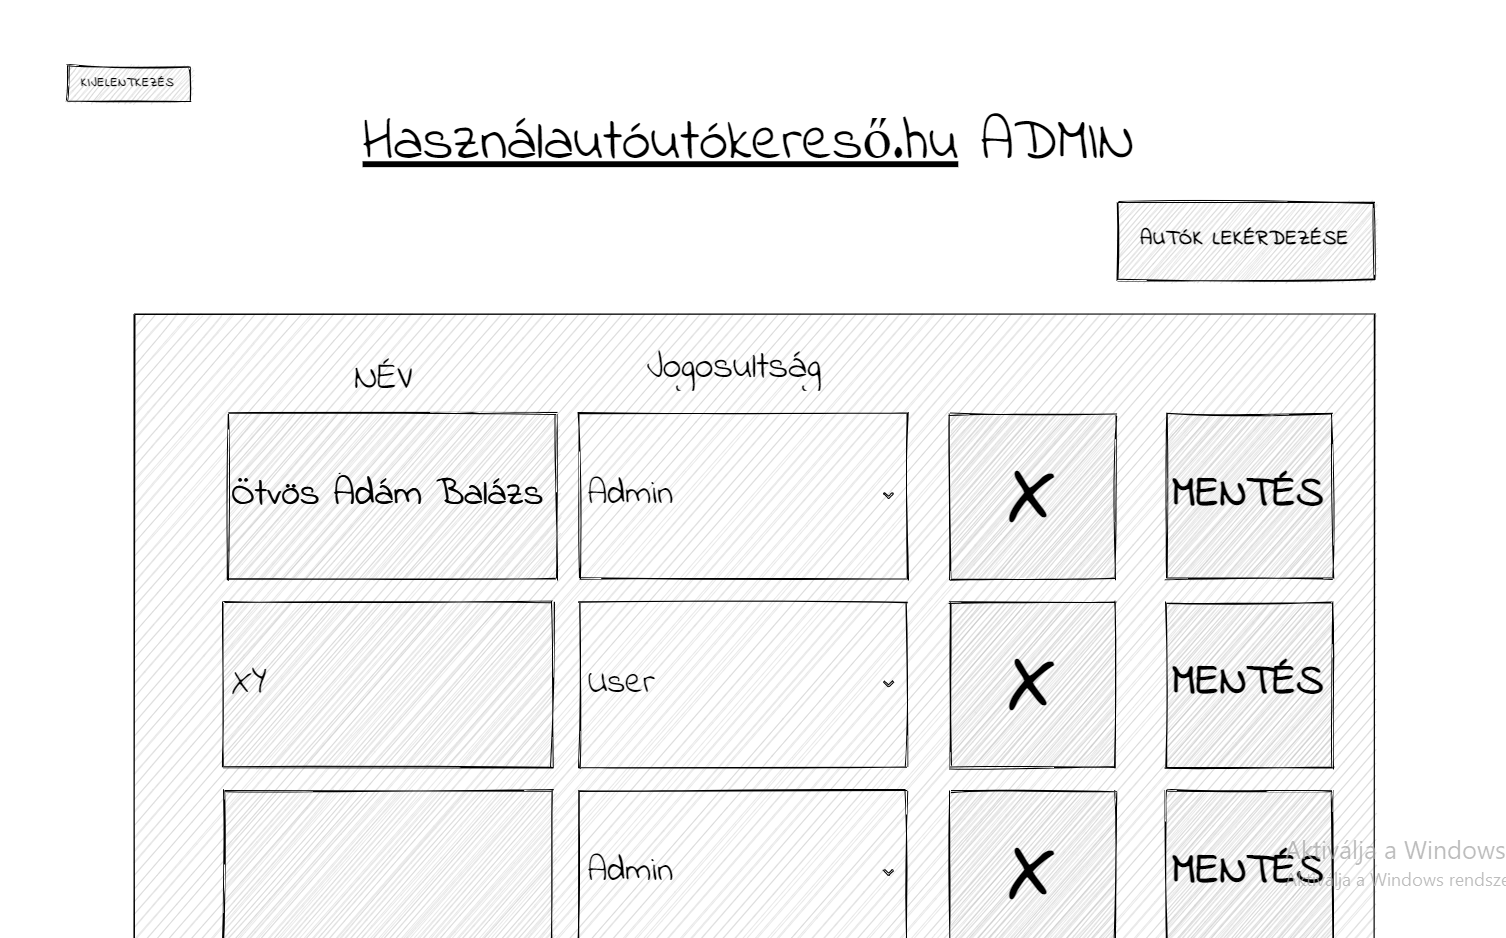
\includegraphics[scale=0.4]{images/Admin.png}}
\caption{Admin oldal}
\label{fig:Admin}
\end{figure}
\newpage

\Section{Adat táblák}

Az alkalmazás elkészítéséhez 3 darab táblára lesz szükség egy
felhasználók(users), autók(cars) és a keresési adatok(search data).

User tábla:
\begin{itemize}
\item Itt lesznek eltárolva a felhasználó adatai a regisztráció után. Ilyen a jelszó a felhasználónév és jogosultsága hogy admin vagy user-e. A jogosultságot az Admin rangú felhasználó tudja változtatni.
\end{itemize}

Cars tábla:
\begin{itemize}
\item Az autók lekérdezése után itt tárolódnak autók és a hozzájuk tartozó adatokat és link ami az autó hirdetésére vezet át
\end{itemize}

Search data tábla:
\begin{itemize}
\item Ez a tábla tárolja a márka nevét és azt az időpontot, amikor csak egy adott márkájú autóra keresnek rá.(Márkára szűrve keresnek)
\end{itemize}
 
 \begin{figure}[h]
\centering
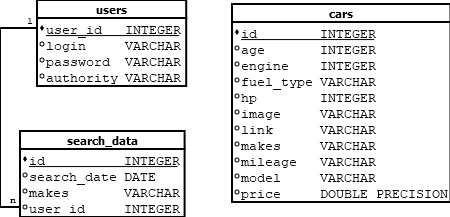
\includegraphics[scale=0.6]{images/Data_Table.png}
\caption{Adatbázis táblák}
\label{fig:DataTable}
\end{figure}

A users és search data tábla között egy-több kapcsolat lesz mivel egy user-hez több keresési előzmény is tartozhat,de egy kereséshez csak egy felhasználó.

A cars tábla független lesz a többitől mivel ide az adatok más oldalról lesznek letöltve és így nem tartozik a user-hez.

 
\Section{API-k megtervezése}
A programban használt Api-król lesz szó ebben a fejezetben
\begin{itemize}
\item /set:

Ha egy Admin frissíteni szeretné az autók tartalmát ez a végpont akkor fog meghívódni.
\item /get

Ha egy felhasználó autóra akar keresni akkor innen fognak lehívódni a megfelelő adatok.
\item /getMakes

Ez az Endpoint akkor fog meghívódni mikor egy felhasználó márkára akar szűrni, hogy lássa milyen márkájú autók találhatóak a weboldalon.
\item /getModels

Márka kiválasztása után automatikusan meghívódik,azért, hogy tudjunk Márkán belül Modellekre is szűrni.

\item /getData

Ha a felhasználó statisztikát szeretne nézni, akkor ez a végpont hívódik majd meg.
\item /postData

Autók lekérdezésének folyamatában fog meghívódni és elmenti azt a Márkát az adatbázisba azzal a dátummal amikor szűrtek rá.
\item /authenticate
Ezen a végponton tud majd bejelentkezni a felhasználó.

\item /register

Regisztráláskor ide küldődik majd el a felhasználó adatai.
\item /users

Itt tudjuk majd lekérdezni az összes felhasználót a hozzá tartózó nevet és jogosultságot.
\item /deleteUser

Ennél a végpontnál tudunk majd felhasználót törölni
\item /updateUser

Ennél  a végpontál tudjuk majd változtatni a felhasználó jogosultságát.

\end{itemize}









